\documentclass[11pt]{article}

% load packages
\usepackage{amsmath}
\usepackage{amssymb}
\usepackage{changepage}
\usepackage{enumitem}
\usepackage{eurosym}
\usepackage{etaremune}
\usepackage{fancyhdr}
\usepackage{fontspec}
\usepackage{geometry}
\usepackage{graphicx}
\usepackage[hidelinks]{hyperref}
\usepackage{lastpage}
\usepackage{longtable}
\usepackage{quoting}
\usepackage{scrextend}
\usepackage{xcolor}
\usepackage{pgfplots}
\pgfplotsset{compat=1.18}
\definecolor{barblue}{HTML}{2A6F97}

% settings for individual packages
\bibliographystyle{acm}
\quotingsetup{vskip=5pt}
\setlist{nosep}
\DeclareMathOperator*{\argmax}{arg\,max}
\DeclareMathOperator*{\argmin}{arg\,min}

% define page size, paragraph indentation, and font
\setlength{\parindent}{0pt}
\setlength{\parskip}{6pt}
\geometry{top=2cm, bottom=2cm, left=2cm, right=2cm, marginparsep=4pt, marginparwidth=1in}

% define the header (empty) and footer (page numbers)
\renewcommand{\headrulewidth}{0pt}
\pagestyle{fancyplain}
\fancyhf{}
\cfoot{\small \thepage\ / \pageref{LastPage}}

% section spacing
\usepackage{titlesec}
\titlespacing*{\section}{0pt}{10pt}{4pt}
\titlespacing*{\subsection}{0pt}{8pt}{2pt}

% start of the document
\begin{document}

\fontsize{10}{13}\selectfont

\vspace*{-30pt}

% start standard header
\begin{center}
{\fontsize{13}{16}\selectfont \textbf{Anthology of Computers and the Humanities}} \\[3pt]
{\fontsize{11}{14}\selectfont Annual Report, 2025--2026} \\[3pt]
Prepared by Taylor Arnold, Editor-in-Chief (\href{mailto:tarnold2@richmond.edu}{tarnold2@richmond.edu}) \\
Submitted to the Advisory Board and the Executive Board of the Association for Computers and the Humanities
\end{center}

\vspace{4pt}
\hrule
\vspace{8pt}

\section*{1.\quad Executive Summary}

The Anthology of Computers and the Humanities completed its first year of operation. In this period the Anthology moved from an idea, approved by the ACH Executive Board, to a working scholarly publisher with a public website, a ratified governance framework, and the full technical and legal infrastructure required for durable, indexed publishing. Over the year we published five volumes containing 143 individual works by 390 distinct authors, drawn from four digital humanities conferences and workshops on two continents, together with an inaugural volume describing the project itself. Each work received a registered DOI and is preserved as both an archival PDF and a searchable HTML page. The Anthology obtained an ISSN from the Library of Congress (ISSN~3070--8931), became a member of CrossRef under its own DOI prefix (\texttt{10.63744}), and built a repeatable metadata-deposit workflow. Beyond its own volumes, the Anthology put this infrastructure to work for the wider community: we used it to retrofit registered DOIs onto the complete twenty-year back catalogue of \textit{Digital Humanities Quarterly} (DHQ), a sibling ACH publication that had never had persistent identifiers for its articles---some 835 articles, now live and resolving through CrossRef. In its first partial year of resolution reporting, the Anthology's DOI prefix already logged more than 47{,}000 successful resolutions. The direct financial cost of the year was small and largely in kind, which makes the Anthology an inexpensive piece of shared infrastructure for ACH to sustain.

\section*{2.\quad Mission and Background}

The Anthology exists to fill a specific gap in digital humanities publishing. Conference proceedings in the field have long lacked a durable, properly indexed home. Organizers have typically had to choose between self-hosting their proceedings, which usually means the papers get no persistent identifiers and no guarantee that they will be preserved or indexed, or fitting their work into the archives of adjacent fields such as the ACL Anthology, the ACM International Conference Proceedings Series, or the IEEE conference archive, none of which were built for the methods and languages of the humanities. As a result, a large share of the field's scholarly conversation has been effectively uncitable and at risk of quiet disappearance once a conference website lapses.

The Anthology addresses that need directly. As set out in its governance document, it is an officially sponsored open platform for peer-reviewed conference and workshop proceedings across the digital humanities, broadly defined: a centralized repository that supports discovery, citation, and long-term preservation. It is modeled on the disciplinary repositories that have served neighboring fields well, but it is designed around the realities of digital humanities work, including multilingual scholarship, a wide range of methods, and conferences that vary greatly in size and format. This mission follows directly from ACH's own work to sustain scholarly infrastructure for the field, and the sections below should be read as progress toward that mission rather than as a list of completed tasks.

\section*{3.\quad Infrastructure and Governance Milestones}

\textbf{Website and platform.} The Anthology launched its public website at \href{https://anthology.ach.org/}{anthology.ach.org}, hosted as a subsite of ACH using the organization's existing GitHub and Reclaim Hosting accounts. Every article is published in two forms: an archival PDF, generated from a shared LaTeX template, and a searchable HTML page for findability. The publishing pipeline, including the LaTeX class, the ingest and build scripts, and the CrossRef metadata generation, is maintained in a single open repository, which makes the operation reproducible and reduces the platform's dependence on any one person.

\textbf{Governance documents.} The Anthology's governance document was drafted on 22 June 2025 and approved by the ACH Executive Board on 28 August 2025. It establishes the mission and scope of the publication, the organizational structure (an Editor-in-Chief serving a single five-year term and a seven-member Advisory Board representing diverse areas of the field), the process by which conferences apply for inclusion, and the editorial model in which each conference retains autonomy over peer review while the Anthology guarantees platform-wide consistency. The document also sets the publication's core policies: open calls for participation, mandatory peer review, publication of original work, a standard Creative Commons Attribution 4.0 International (CC~BY~4.0) license with copyright retained by authors, article-removal and retraction procedures, and the commitment to persistent identifiers and indexing. These policies are summarized publicly on the Anthology's About page and govern every volume.

\textbf{Persistent identifiers and indexing.} The Anthology joined CrossRef and registers a DOI for every published work under its own prefix (\texttt{10.63744}); as of this report, all 143 published works resolve through CrossRef. Metadata is deposited using CrossRef's version 4.4.2 schema through a scripted workflow that generates a validated XML deposit for each volume from the same source data used to build the site, which keeps the public record and the registered metadata in sync. The publication received its ISSN, 3070--8931, from the Library of Congress. The platform supports ORCID identifiers for authors, in line with the governance commitment to persistent author identification, and ORCID coverage is expected to grow as adoption increases among contributors.

\section*{4.\quad Publications}

The Anthology published five volumes in its first year. Volume~1 is an inaugural volume containing a single article by the Editor and Advisory Board that introduces the platform and its rationale; it doubles as field-facing scholarship about the publishing model itself and is worth highlighting on that basis. Volumes~2 through~5 are peer-reviewed proceedings from four distinct conferences and workshops, including one Francophone volume, which demonstrates the platform's multilingual reach. Table~\ref{tab:vols} summarizes the year's output.

\begin{table}[h]
\centering
\small
\begin{tabular}{p{0.7cm} p{7.7cm} p{1.4cm} p{1.2cm} p{1.4cm}}
\hline
\textbf{Vol.} & \textbf{Source / Conference} & \textbf{Date} & \textbf{Works} & \textbf{Authors} \\
\hline
1 & Inaugural volume (about the Anthology) & Sep 2025 & 1 & 8 \\
2 & Digital Humanities Tech Symposium 2025 (DH2025, Lisbon) & Oct 2025 & 8 & 14 \\
3 & Computational Humanities Research 2025 (CHR, Luxembourg) & Nov 2025 & 97 & 280 \\
4 & Actes de la Conf\'erence Humanistica 2026 (Paris) & May 2026 & 27 & 82 \\
5 & From Manuscript to Megabyte / DHCNC 2026 (North Carolina) & Jul 2026 & 10 & 19 \\
\hline
& \textbf{Total} & & \textbf{143} & \textbf{390*} \\
\hline
\end{tabular}
\caption{Volumes published in 2025--2026. ``Works'' includes editors' introductions where present. *The author total is de-duplicated across all volumes, so it is smaller than the sum of the per-volume counts.}
\label{tab:vols}
\end{table}

The volumes span a wide methodological and geographic range: the technical and research-software focus of the Digital Humanities Tech Symposium held at DH2025 in Lisbon; the large computational-methods program of Computational Humanities Research, held at the Luxembourg Centre for Contemporary and Digital History (C2DH) and by itself accounting for 97 works; the Francophone scholarship of the Humanistica proceedings from Paris; and the preservation- and sustainability-themed institute From Manuscript to Megabyte, organized with North Carolina State University Libraries.

\textbf{Usage data.} The Anthology now has its first meaningful window of DOI-resolution data from CrossRef. CrossRef reports resolution activity for the whole \texttt{10.63744} prefix, which covers both the Anthology's own volumes and the retrofitted \textit{Digital Humanities Quarterly} back catalogue (Section~5). From the first recorded activity in September 2025 through June 2026, the prefix received 57{,}138 resolution attempts, of which 47{,}143 (about 83\%) resolved successfully at CrossRef; the balance are lookups for DOIs that had been requested but not yet deposited, together with occasional technical failures. Monthly volume grew from a handful of resolutions at launch to 11{,}133 attempts and 10{,}863 successful resolutions in June 2026 alone---a month-level success rate of 97.6\% across 1{,}077 unique DOIs. Figure~\ref{fig:resolutions} shows successful resolutions by month over the reporting window.

These figures cover the twelve-month reporting window and therefore exclude Volume~5, which was published in July 2026, after the window closed; its resolution activity will first appear in next year's report. As Table~\ref{tab:resbytitle} shows, the large majority of current traffic is to DHQ articles rather than to the Anthology's own volumes, which is expected: DHQ represents roughly two decades of accumulated, widely cited scholarship, whereas the Anthology's volumes are new and still building an audience. We will continue to pair these resolution reports with server-side page and PDF request logs so that next year's report can present a clean year-over-year comparison from this baseline. Establishing that baseline was itself a first-year deliverable.

\begin{figure}[h]
\centering
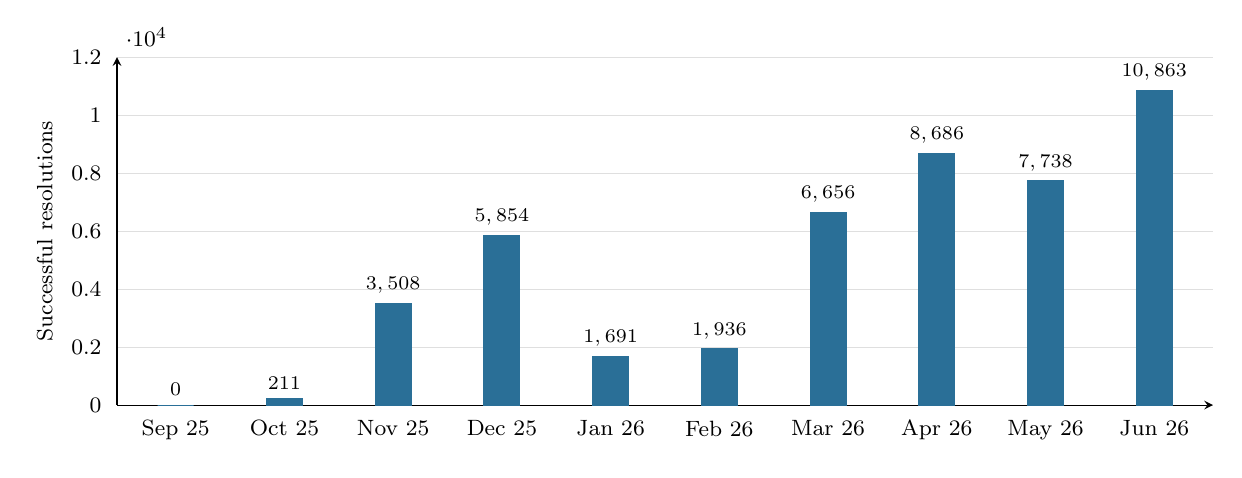
\begin{tikzpicture}
\begin{axis}[
    width=15.5cm, height=6cm,
    ybar,
    bar width=13pt,
    ymin=0, ymax=12000,
    ytick={0,2000,4000,6000,8000,10000,12000},
    yticklabel style={/pgf/number format/1000 sep={,}, font=\footnotesize},
    ylabel={Successful resolutions},
    ylabel style={font=\footnotesize},
    symbolic x coords={Sep 25,Oct 25,Nov 25,Dec 25,Jan 26,Feb 26,Mar 26,Apr 26,May 26,Jun 26},
    xtick=data,
    xticklabel style={font=\footnotesize},
    nodes near coords,
    nodes near coords style={font=\scriptsize, /pgf/number format/1000 sep={,}},
    every node near coord/.append style={anchor=south},
    axis lines=left,
    ymajorgrids=true,
    major grid style={line width=0.3pt, draw=gray!25},
    tick style={draw=none},
    enlarge x limits=0.06,
    clip=false,
]
\addplot[fill=barblue, draw=barblue] coordinates {
    (Sep 25,0) (Oct 25,211) (Nov 25,3508) (Dec 25,5854) (Jan 26,1691)
    (Feb 26,1936) (Mar 26,6656) (Apr 26,8686) (May 26,7738) (Jun 26,10863)
};
\end{axis}
\end{tikzpicture}
\caption{Successful DOI resolutions per month for the Anthology's \texttt{10.63744} prefix, September 2025 through June 2026 (CrossRef resolution report). Counts cover both the Anthology's own volumes and the retrofitted DHQ back catalogue. There was no recorded resolution activity before September 2025, and Volume~5 (July 2026) falls outside this window.}
\label{fig:resolutions}
\end{figure}

\begin{table}[h]
\centering
\small
\begin{tabular}{p{9cm} r r}
\hline
\textbf{Publication title} & \textbf{Resolutions} & \textbf{Unique DOIs} \\
\hline
\textit{Digital Humanities Quarterly} (DHQ retrofit) & 8,942 & 835 \\
Computational Humanities Research 2025 (Vol.~3) & 1,375 & 97 \\
Actes de la Conf\'erence Humanistica 2026 (Vol.~4) & 432 & 27 \\
Digital Humanities Tech Symposium 2025 (Vol.~2) & 82 & 8 \\
Inaugural Volume (Vol.~1) & 32 & 1 \\
\hline
\textbf{Total} & \textbf{10,863} & \textbf{968} \\
\hline
\end{tabular}
\caption{Successful DOI resolutions by publication for the most recent reporting month (June 2026), from the CrossRef resolution report. Volume~5 does not appear because it was published in July 2026, after the reporting window.}
\label{tab:resbytitle}
\end{table}

\section*{5.\quad Service to the Field: The DHQ DOI Retrofit}

The clearest evidence that the Anthology's infrastructure benefits the wider ACH ecosystem is the \textit{Digital Humanities Quarterly} (DHQ) project. DHQ is a long-running, open-access ACH journal whose articles, published over roughly two decades, had never been assigned DOIs. Without persistent identifiers, two decades of scholarship was harder to cite reliably, was not linked into the CrossRef citation graph, and was vulnerable to link rot.

Using the same CrossRef membership, metadata tooling, and deposit workflow built for the Anthology's own volumes, we retrofitted registered DOIs onto DHQ's complete back catalogue: 835 articles spanning roughly two decades of publication (2007--2026). The work involved assembling and normalizing metadata for the full run, generating schema-valid CrossRef deposits, and reconciling the results, and it was carried out with modest volunteer labor measured in days rather than months because the tooling already existed. The outcome is that every DHQ article now has a persistent, resolvable identifier and is registered in CrossRef at no new membership cost to ACH. This project deserves emphasis: it shows that a single shared piece of infrastructure, built once for the Anthology, can be reused to solve adjacent problems across ACH's publications.

The retrofit is already in active use, and the resolution data makes this concrete. In June 2026 alone, DHQ DOIs drew 8,942 successful resolutions---about 82\% of all resolution traffic on the Anthology's prefix that month (Table~\ref{tab:resbytitle})---and every one of the 835 articles resolved at least once during the month. In other words, the identifiers are not merely registered but live, discoverable, and being followed across the full run of the journal. Two decades of DHQ scholarship that had previously sat outside the CrossRef citation graph is now linked into it.

\section*{6.\quad People}

The Anthology is run by a small group of volunteers. The Editor-in-Chief, Taylor Arnold (University of Richmond), is responsible for accepting volume proposals, operating the publishing platform, and depositing metadata with CrossRef. Long-term planning is shared with the Advisory Board, whose current members are:

\begin{itemize}[leftmargin=1.5em]
\item Maria Antoniak, University of Colorado, U.S.A.
\item Miguel Escobar Varela, National University of Singapore
\item Mila Oiva, University of Turku, Finland
\item Marie Puren, EPITA, Paris, France
\item Amanda Regan, Clemson University, U.S.A.
\item Melanie Walsh, University of Washington, U.S.A.
\end{itemize}

Under the Anthology's editorial model, the substantive editorial labor for each volume, including running the call for papers, managing peer review, and making acceptance decisions, is carried out by the program chairs of each conference, who serve as volume editors. In the first year these volume editors were: Julia Damerow and Rebecca Sutton Koeser (Volume~2); Taylor Arnold, Margherita Fantoli, and Ruben Ros (Volume~3); Serena Crespi, Simon Gabay, Martin Grandjean, Ariane Pinche, Marie Puren, and L\'ea Saint-Raymond (Volume~4); and James B. Harr~III, Emma Stanley, Jenna Rinalducci, and Donna Kain (Volume~5). Beyond these named editors, the peer review that underpins each volume was performed by the conferences' own reviewer pools, representing a substantial amount of uncompensated community labor. The Anthology also works closely with the ACH Executive Board, which sponsors and funds the CrossRef membership.

A note on sustainability: the current model concentrates platform operations and all CrossRef deposits in a single Editor. This is efficient and inexpensive, but it is a concentration of institutional knowledge that the Anthology should reduce over time through documentation and, eventually, additional technical contributors.

\section*{7.\quad Finances and Resources}

The Anthology's direct costs in its first year were small and were met by ACH and by in-kind contributions.

\begin{itemize}[leftmargin=1.5em]
\item \textbf{CrossRef membership and DOI registration.} Covered by the ACH Treasurer under the commitment in the governance document to fund the direct costs of CrossRef membership, expected to be about \$1{,}000 per fiscal year. DOI registration fees for the Anthology's own volumes and for the DHQ retrofit fall under this membership.
\item \textbf{Hosting.} Effectively zero incremental cost. The website runs on ACH's existing GitHub and Reclaim Hosting accounts as a subsite, so no separate hosting contract was required.
\item \textbf{Labor.} Entirely volunteer and in-kind: the Editor's platform work, the volume editors' peer-review and editorial work, and the Advisory Board's oversight. No stipends or salaries were paid.
\end{itemize}

In sum, the Anthology delivered five volumes, 143 registered works, and the DHQ retrofit for roughly \$1{,}000 in cash outlay. That efficiency depends on volunteer time, which should be counted as a real cost when planning for growth, even though no money changed hands for it this year.

\section*{8.\quad Challenges and Lessons Learned}

The first year surfaced friction worth recording honestly. The largest recurring cost was metadata: source material arrives from each conference in inconsistent shape, and cleaning author names, affiliations, and titles into schema-valid CrossRef deposits took more effort than any other single task. Small artifacts (duplicated author entries, stray markup in names, inconsistent handling of non-English characters) are easy to introduce and tedious to catch, and they argue for tighter validation earlier in the pipeline and clearer submission guidance for volume editors. Onboarding conference organizers also takes lead time: the governance document asks for an email of interest ideally two months before a call for papers, and the volumes that went most smoothly were those where that conversation happened early. Finally, the concentration of the workflow in one person, noted above, is convenient but fragile. None of these problems threatened the year's output, but each points to concrete process improvements for year two.

\section*{9.\quad Goals for Year Two}

\begin{itemize}[leftmargin=1.5em]
\item \textbf{Recruit new volumes.} Continue converting expressions of interest into published volumes, with a particular focus on recurring conference series that would benefit from a stable annual home, and on broadening linguistic and regional coverage beyond the first year's mix.
\item \textbf{Expand indexing.} Pursue inclusion in the Directory of Open Access Journals (DOAJ) now that an ISSN, a public license, and a peer-review policy are in place, and evaluate the longer-term path toward broader scholarly indexes such as Scopus as the publication accumulates a track record.
\item \textbf{Formalize preservation.} Move from ``preserved as PDF and HTML in a public repository'' to a formal digital-preservation arrangement, evaluating LOCKSS, CLOCKSS, or Portico so that long-term preservation does not depend solely on the ACH-hosted site.
\item \textbf{Improve search and discovery.} Strengthen on-site search across the full corpus and ensure the HTML and metadata are well exposed to external discovery services.
\end{itemize}

\end{document}
